% ------------------------------------------------------------------------------------------------
% Section 8.3 of the Heston report : static no-arbitrage conditions.
% Paste in place of the empty subsections 8.3.1 - 8.3.3. Requires \usepackage{booktabs} and \usepackage{graphicx}.
% Figures : generated by make_no_arbitrage_figures.py into figures/ (adapt the paths to your figure folder).
% Numbers : section 8 of Model/heston_test.ipynb.
% ------------------------------------------------------------------------------------------------
\subsection{No-Arbitrage conditions}
In this section, we check whether the interpolated implied volatility surfaces and the Heston prices satisfy the
three static no-arbitrage conditions of Section~2.2. With the moneyness $\kappa = K/F(T)$ and the normalised call
price $\hat c(\kappa, T) = C(\kappa F(T), T) / (D(T) F(T))$, we have $\partial_K C = D(T)\,\partial_\kappa \hat c$, and the
conditions read
\begin{equation}
-1 \le \partial_\kappa \hat c(\kappa, T) \le 0, \qquad \partial_{\kappa\kappa} \hat c(\kappa, T) \ge 0, \qquad
T \mapsto \hat c(\kappa, T) \ \text{non-decreasing at fixed } \kappa .
\end{equation}
On a discrete grid of strikes they are exactly conditions on the slopes between neighbouring points: slopes in
$[-1, 0]$ (monotonicity), non-decreasing slopes (butterfly), and prices non-decreasing from one maturity to the next
(calendar). They are checked on a grid of 71 log-moneynesses $k = \ln\kappa \in [-40\%, 30\%]$ (step 1\%) and 61
maturities (the 13 listed expiries and 48 dates in between), i.e. 4{,}270 monotonicity, 4{,}209 butterfly and 4{,}260
calendar tests per surface. For an implied volatility surface,
$\hat c = N(d_1) - \kappa N(d_2)$, $d_{1,2} = -\ln\kappa / \sqrt{w} \pm \sqrt{w}/2$, $w = \sigma^2 T$. A violation is counted
when a condition fails by more than $10^{-7}$, i.e. 0.0008 index point on a forward of 8000.

Six surfaces are checked: the market surface interpolated linearly in strike and in total variance across expiries
(V2T, the interpolation of Figure~5), by SVI slices and by SSVI (Section~7.5); the Heston prices of the Lewis formula,
with the quadrature of Section~5.3 (4{,}000 nodes up to $u = 1000$) and with a fine one (60{,}000 nodes up to
$u = 3000$); and the Heston implied surface interpolated like the market one. Table~\ref{tab:no_arbitrage} gives the
results and Figure~\ref{fig:no_arbitrage_map} the location of the violations.

\begin{table}[h]
\centering
\begin{tabular}{@{}lrrrrrr@{}}
\toprule
 & \multicolumn{2}{c}{\textbf{Monotonicity}} & \multicolumn{2}{c}{\textbf{Butterfly}} & \multicolumn{2}{c}{\textbf{Calendar}} \\
\cmidrule(lr){2-3}\cmidrule(lr){4-5}\cmidrule(lr){6-7}
\textbf{Surface} & \textbf{viol.} & \textbf{worst} & \textbf{viol.} & \textbf{worst} & \textbf{viol.} & \textbf{worst} \\
\midrule
Market, linear + V2T & 0 & -- & 139 & $1.2 \times 10^{-1}$ & 0 & -- \\
Market, SVI & 1 & $5.6 \times 10^{-4}$ & 0 & -- & 12 & $1.0 \times 10^{-3}$ \\
Market, SSVI & 0 & -- & 0 & -- & 0 & -- \\
Heston, default quadrature & 45 & $3.5 \times 10^{-6}$ & 0 & -- & 0 & -- \\
Heston, fine quadrature & 0 & -- & 0 & -- & 0 & -- \\
Heston implied, linear + V2T & 0 & -- & 107 & $7.1 \times 10^{-2}$ & 0 & -- \\
\bottomrule
\end{tabular}
\caption{Static no-arbitrage violations on a grid of 71 log-moneynesses and 61 maturities. Worst: largest violation of
the normalised condition (slope outside $[-1, 0]$, decrease of the slope, decrease of $\hat c$ in $T$).}
\label{tab:no_arbitrage}
\end{table}

\begin{figure}[h]
\centering
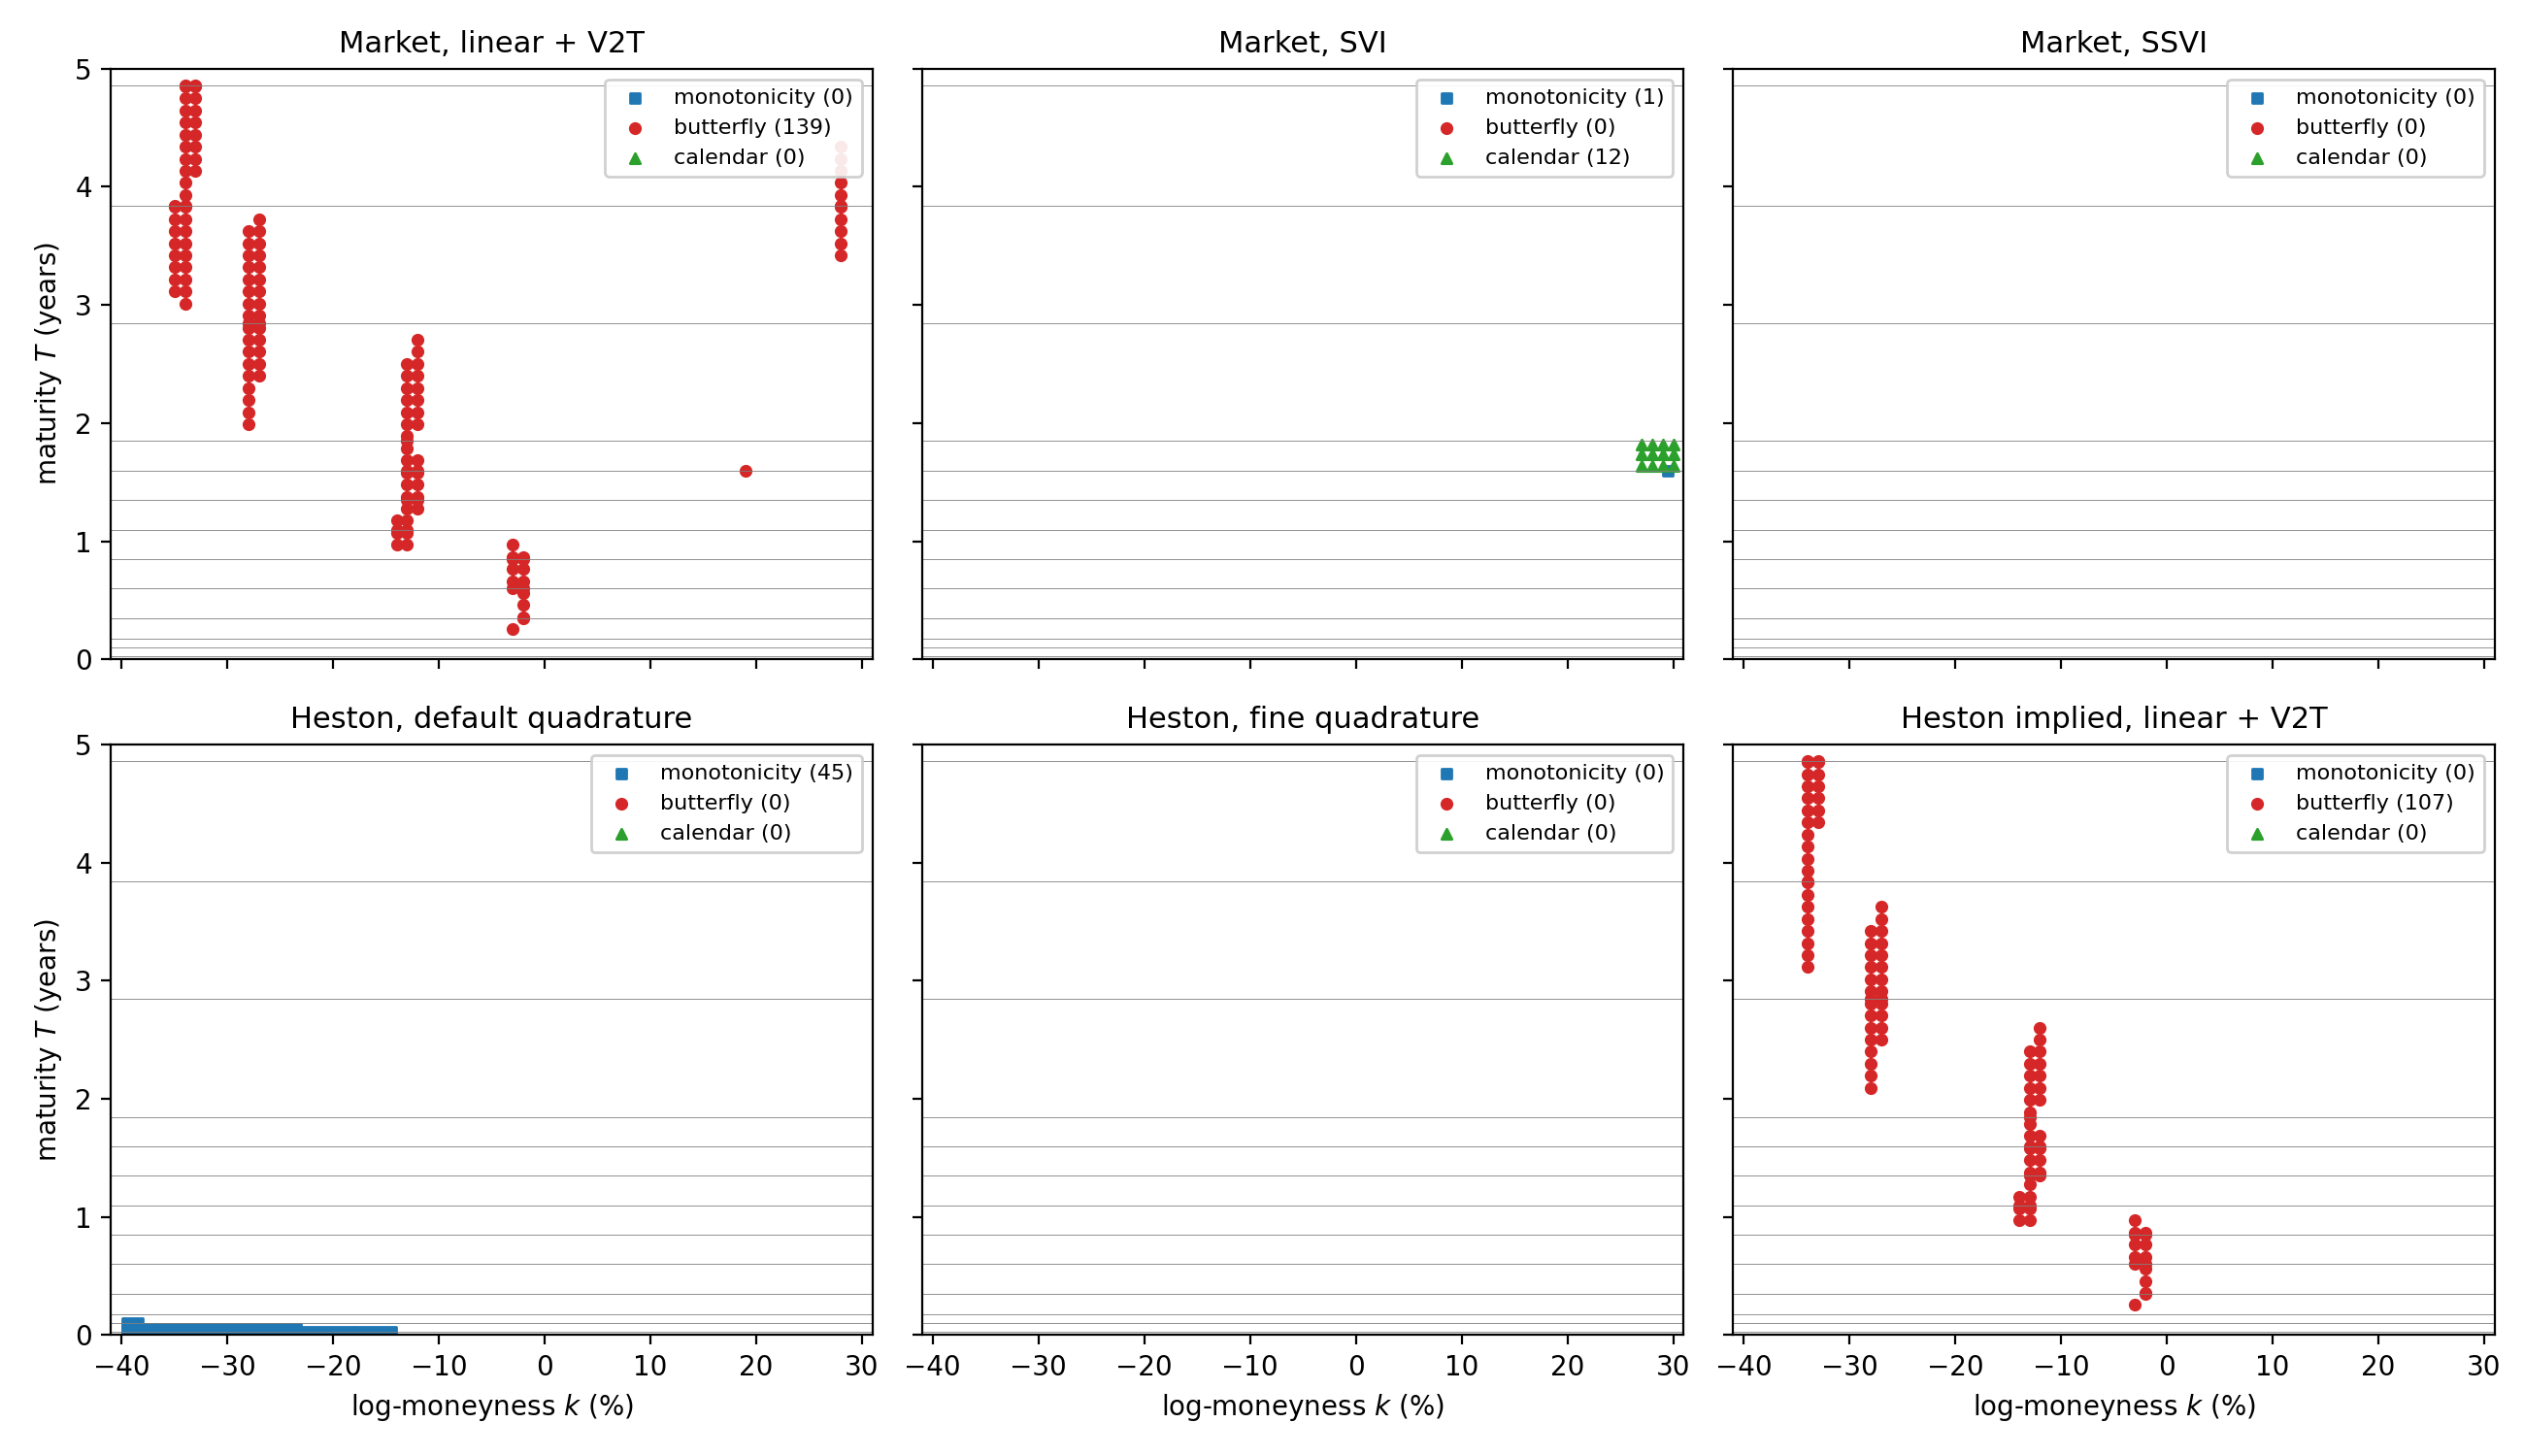
\includegraphics[width=\textwidth]{figures/no_arbitrage_map.png}
\caption{Location of the violations in the $(k, T)$ plane (horizontal lines: listed expiries).}
\label{fig:no_arbitrage_map}
\end{figure}

\subsubsection{Monotonicity}
The interpolated market surfaces satisfy the monotonicity condition everywhere except at one point of the SVI surface,
at $T = 1.60$ and $k = 29.5\%$, where the crossing of two SVI slices described in Section~\ref{sec:calendar_check} also
produces a call price slightly increasing in strike. The Heston model is free of arbitrage by construction, yet the
default quadrature gives 45 violations, all at $T \le 0.1$ year and $k \le -14\%$. There, the out-of-the-money prices are
almost zero and the truncation of the Lewis integral leaves an error of about $-6 \times 10^{-6}$ of the forward (0.05
index point, the order of magnitude found in Section~5.3): Figure~\ref{fig:monotonicity} shows that the default quadrature
even gives slightly negative put prices, while the fine quadrature does not. With the fine quadrature, no violation is
left.

\begin{figure}[h]
\centering
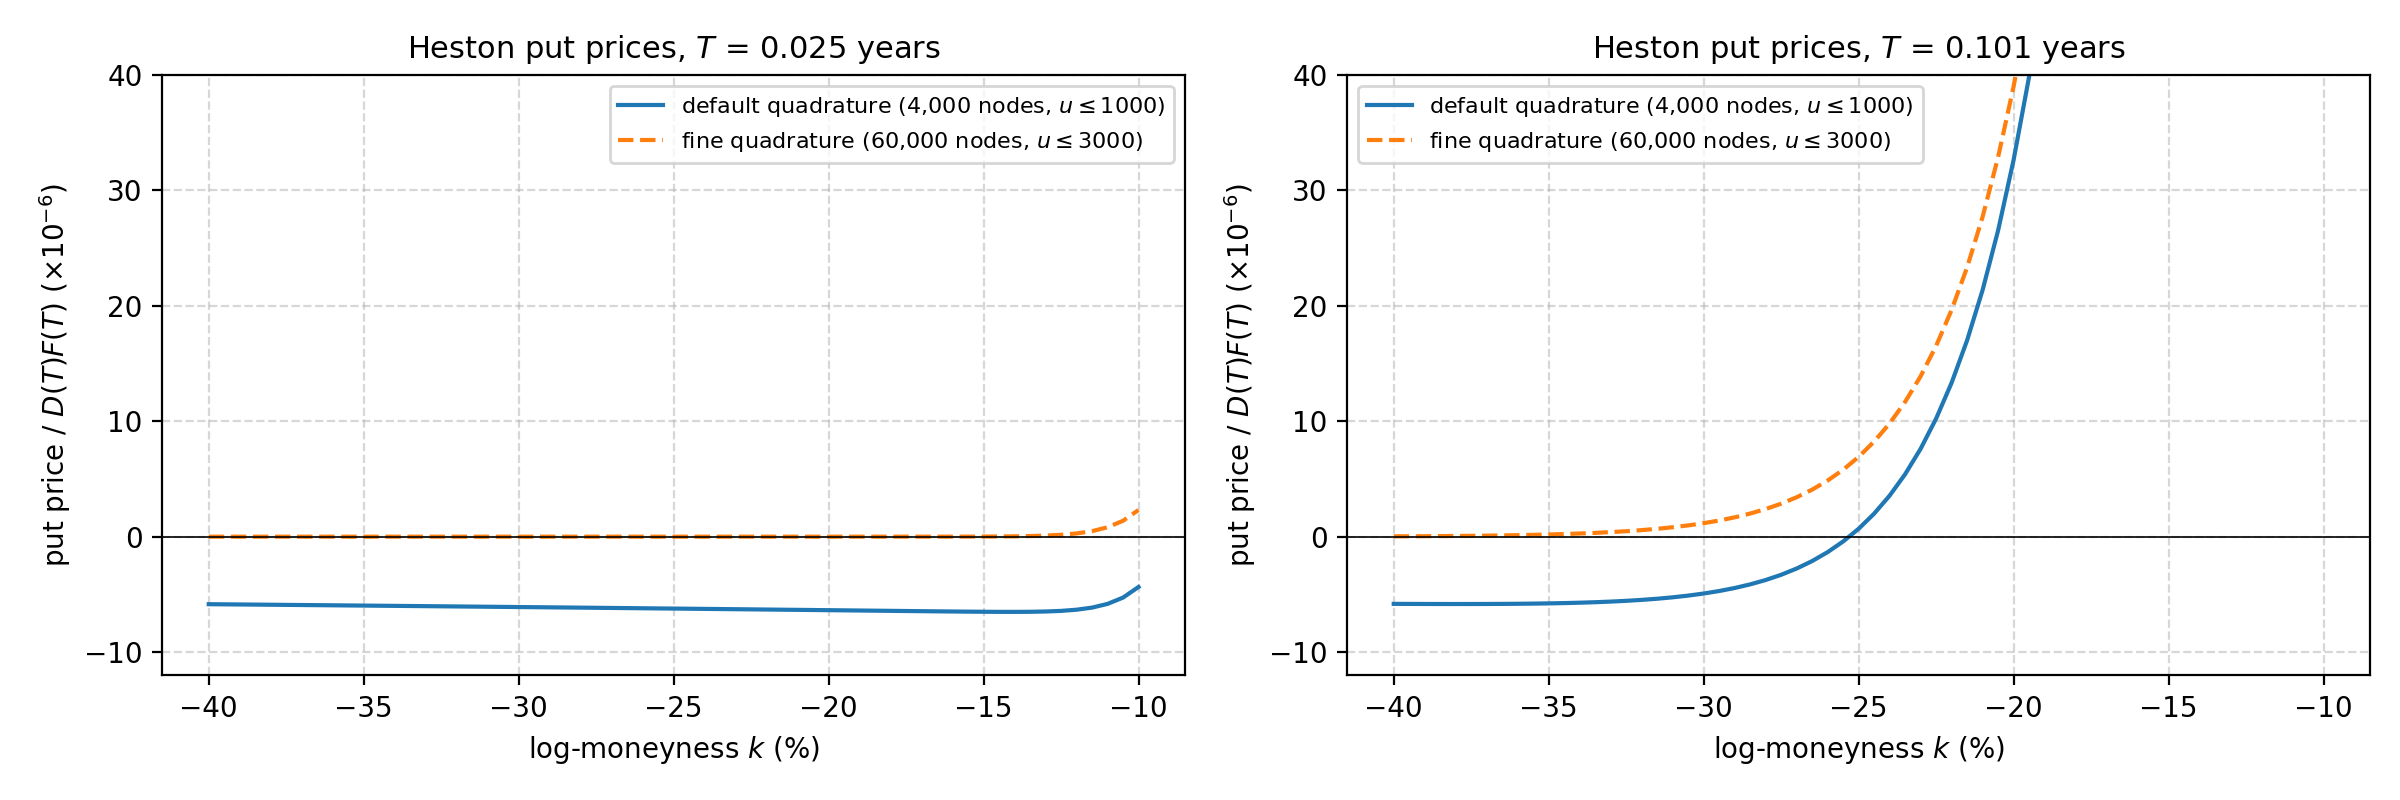
\includegraphics[width=\textwidth]{figures/monotonicity_quadrature.png}
\caption{Heston put prices (normalised) of the far left wing at 9 days and 1 month: the default Lewis quadrature leaves an
error of about $-6 \times 10^{-6}$ of the forward, the fine quadrature none.}
\label{fig:monotonicity}
\end{figure}

\subsubsection{Butterfly}
By the Breeden--Litzenberger identity, the butterfly condition is the positivity of the risk-neutral density
$\partial_{\kappa\kappa}\hat c$ (Figure~\ref{fig:butterfly}). SVI, SSVI and the Heston prices satisfy it everywhere. The linear
interpolation in strike violates it at 139 points (107 on the Heston implied surface), along vertical lines at
$k \approx -35\%, -27\%, -13\%$ and $-3\%$ (Figure~\ref{fig:no_arbitrage_map}). Each line is the lowest quoted strike of a
group of expiries (7800 from 3 to 10 months, 7000 from 1 to 1.8 years, 6000 and 5600 beyond): there, the interpolation
switches from a linear volatility with a negative slope to a flat extrapolation, and the kink makes the density
negative, down to $-15$ at 3.8 years. The linear interpolation also has a kink at every quoted strike, visible as spikes
of the density. Since the Heston implied surface comes from an arbitrage-free model, its 107 violations show that they
are created by the interpolation and not by the data.

\begin{figure}[h]
\centering
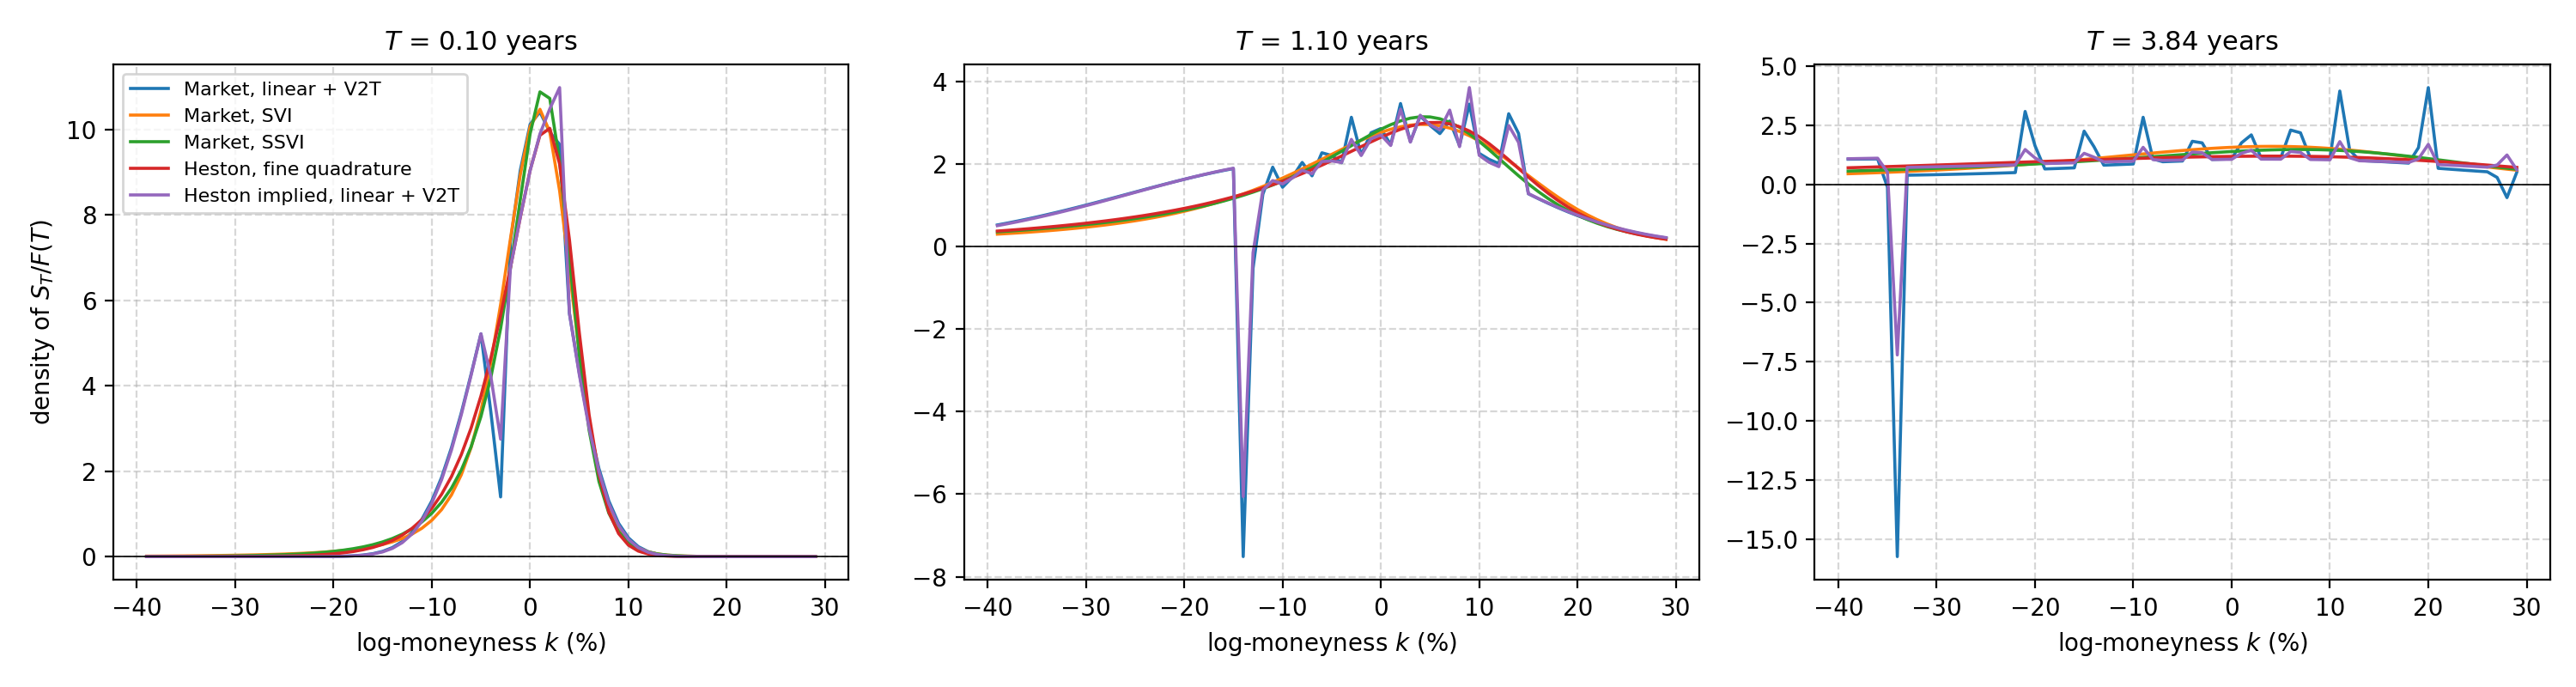
\includegraphics[width=\textwidth]{figures/butterfly_densities.png}
\caption{Risk-neutral densities of $S_T/F(T)$ at 1 month, 1.1 years and 3.8 years.}
\label{fig:butterfly}
\end{figure}

\subsubsection{Calendar}\label{sec:calendar_check}
The linear interpolation in total variance across expiries keeps the calendar condition between the listed expiries,
and SSVI satisfies it by construction ($\theta_T$ non-decreasing). The SVI slices are calibrated independently: the
slices of 1.60 and 1.85 years cross in the right wing (the 1.60-year slice has a positive skew parameter
$\rho = 0.78$, Section~7.5.3), so that the normalised call price decreases between the two expiries for $k \ge 27\%$
(12 violations, Figure~\ref{fig:calendar}). Fitting the slices independently does not guarantee the calendar condition;
SSVI, or SVI slices fitted under calendar constraints, does.

\begin{figure}[h]
\centering
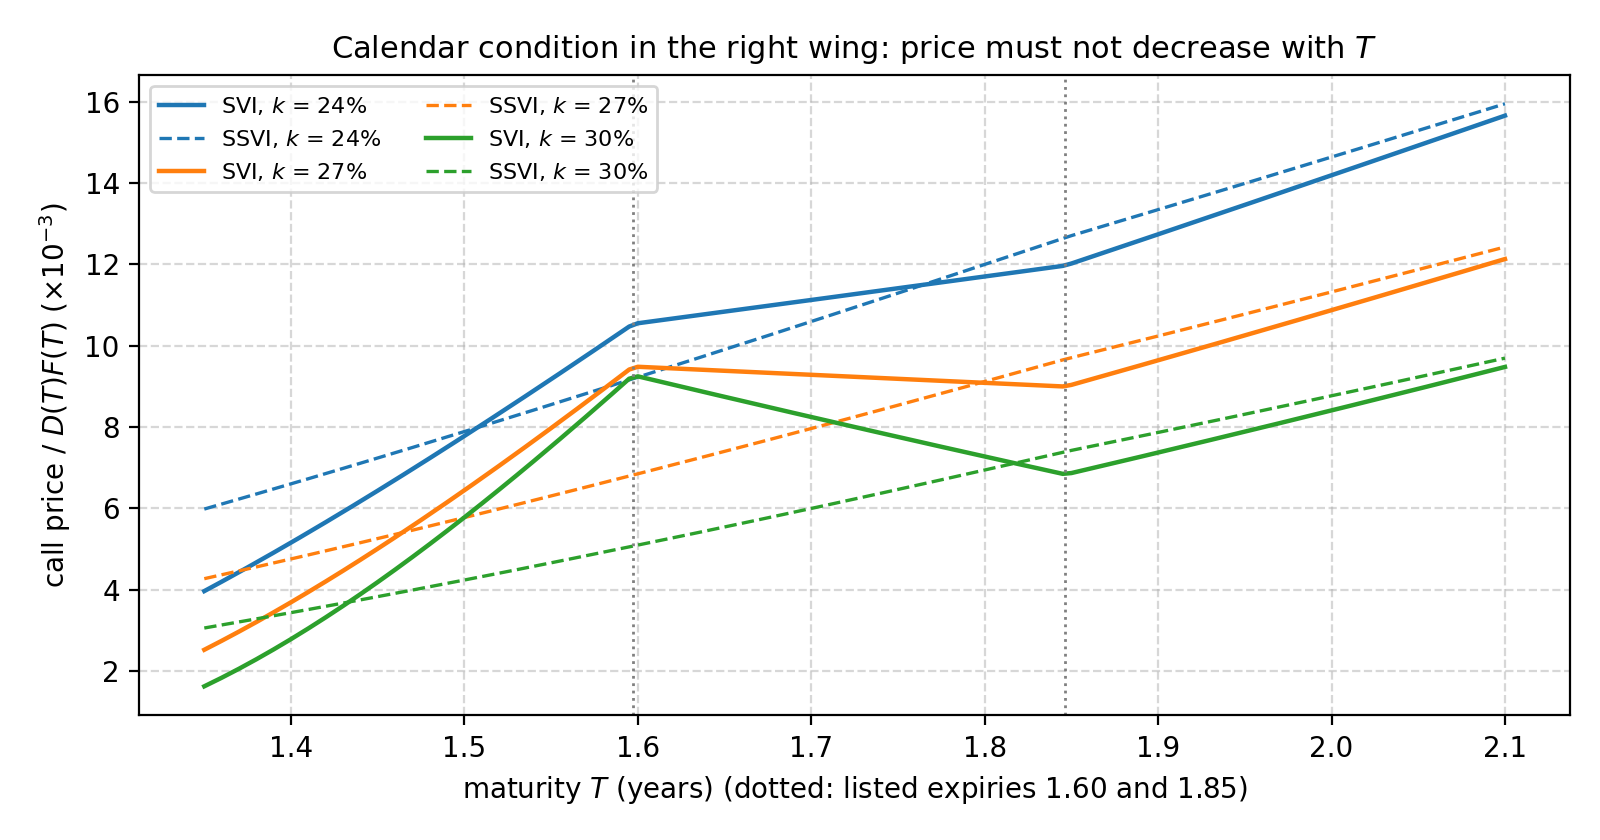
\includegraphics[width=0.8\textwidth]{figures/calendar_svi.png}
\caption{Normalised call prices of the right wing as functions of the maturity: the SVI price decreases between the
1.60 and 1.85-year expiries for $k \ge 27\%$, the SSVI price does not.}
\label{fig:calendar}
\end{figure}

\paragraph{Conclusion.} SSVI is the only interpolation of the market quotes free of static arbitrage on the whole grid.
The linear interpolation in strike, used for the plots of this paper, is adequate for display but creates butterfly
arbitrage at the edges of the quoted strikes: it must not be used to price with a local volatility model, which needs
the second derivative in strike.
